% Written report for the intrusion detection project.
%
% Every number and every figure in this document is produced by a command in
% the repository, listed in the appendix. Nothing is typed in by hand, so the
% paper and the dashboard cannot drift apart.
%
% Build with:  pdflatex -output-directory=build main.tex   (twice)
% or:          python -m ids.report.build

\documentclass[9pt,a4paper,twocolumn]{article}

\usepackage[utf8]{inputenc}
\usepackage[T1]{fontenc}
% A scalable font. Without one, microtype cannot expand and pdflatex stops
% rather than falling back.
\usepackage{lmodern}
\usepackage[english]{babel}
\usepackage[
  a4paper,
  top=18mm, bottom=20mm, left=16mm, right=16mm,
  columnsep=6mm
]{geometry}
\usepackage{graphicx}
\usepackage{booktabs}
\usepackage{caption}
\usepackage{titlesec}
\usepackage[protrusion=true,expansion=false]{microtype}
\usepackage{xcolor}
% Coloured rather than hidden, so a figure or table number reads as something
% that can be clicked and jumps to it.
\usepackage[
  colorlinks=true,
  linkcolor=accent,
  urlcolor=accent,
  citecolor=accent
]{hyperref}
\usepackage{fancyhdr}
\usepackage{amsmath}
\usepackage{siunitx}

\sisetup{group-separator={,}, group-minimum-digits=4}

\definecolor{accent}{HTML}{1F4E9C}

\captionsetup{font=small, labelfont={bf,color=accent}, skip=4pt}
\titleformat{\section}{\normalfont\bfseries\color{accent}}{\thesection}{0.6em}{}
\titleformat{\subsection}{\normalfont\bfseries}{\thesubsection}{0.6em}{}
\titlespacing*{\section}{0pt}{8pt}{4pt}
\titlespacing*{\subsection}{0pt}{6pt}{3pt}

\pagestyle{fancy}
\fancyhf{}
\fancyfoot[C]{\small\thepage}
\renewcommand{\headrulewidth}{0pt}

\setlength{\parskip}{2pt}
\setlength{\columnsep}{6mm}

\title{\vspace{-8mm}\bfseries Three detectors on the same traffic:\\
a comparison of supervised and unsupervised\\
intrusion detection on CICIDS2017}
\author{Youcef Amar\\
\small MSc Cybersecurity, EPFL\\
\small \href{https://github.com/2Fick/AI-Powered-IDS}{github.com/2Fick/AI-Powered-IDS}}
\date{\small\today}

\begin{document}
\maketitle

\begin{abstract}
\noindent\small
A random forest, an isolation forest and a dense autoencoder are trained on the
CICIDS2017 network capture and served behind one API that scores flows one at a
time. The supervised model reaches \SI{99.87}{\percent} recall at a
\SI{0.07}{\percent} false positive rate and decides in \SI{1.66}{\milli\second},
and this report is mostly about why that number should not be read on its own.
Three results qualify it. A random train and test split leaves
\SI{27.8}{\percent} of the test attacks with a byte identical twin in the
training half, though a time ordered split shows the supervised model survives
this while the unsupervised ones lose half their recall. Hyperparameter sweeps
show the forest reaches its recall at five trees and that the scikit-learn
default for the isolation forest sits near the worst end of its own curve.
Removing one attack family from training at a time shows the supervised model
does not degrade gracefully on an unseen family, it collapses to zero on three
of six, and that the unsupervised models recover a third of the loss on two
families and nothing on the rest.
\end{abstract}

\section{Introduction}

Intrusion detection on CICIDS2017 is a solved problem by the usual measure.
Published results routinely report accuracy above \SI{99}{\percent}, and a
random forest fitted in a few minutes reproduces them. That makes the headline
number an uninteresting thing to report and an easy thing to overstate.

This project therefore compares three detectors that answer the same question
in different ways, and spends most of its effort on what qualifies the result
rather than on the result itself.

\begin{itemize}\itemsep1pt
  \item A \textbf{random forest}, supervised, learns from labelled attacks.
  \item An \textbf{isolation forest}, unsupervised, is fitted on benign traffic
        and scores how easily a flow is isolated from the rest.
  \item An \textbf{autoencoder}, unsupervised, is fitted on benign traffic and
        scores how badly it fails to rebuild a flow.
\end{itemize}

All three are served by one FastAPI application, and a dashboard replays held
out traffic through them at a controlled rate so that latency and detection can
be watched rather than quoted.

\section{Data and preprocessing}

\subsection{Which release, and why}

CICIDS2017 is five working days of traffic from a test bed at the University of
New Brunswick, captured in July 2017 with real attacks run against real
machines. It ships in two forms. The widely used \emph{machine learning} CSVs
keep 78 flow statistics and the label, and drop the addresses. The
\emph{labelled flow} release keeps the same statistics and adds flow identity:
source and destination address, ports, protocol and timestamp.

This project uses the second. Without addresses the threat intelligence
enrichment would have nothing real to look up, and without timestamps there is
no capture order to replay. The feature set handed to the models is unchanged.

\subsection{What the raw files actually contain}

Reading the eight capture files before modelling anything turned up four
problems that each changed a decision downstream.

\textbf{Padding rows.} The Thursday morning file carries
\num{288602} rows in which every single column is empty. They have no label, so
a naive reading counts all of them as attacks, which would have shifted the
class balance by ten percentage points.

\textbf{Infinities.} \num{4376} values are infinite, all in
\texttt{Flow Bytes/s} and \texttt{Flow Packets/s}, produced when a flow lasts
zero microseconds and the generator divides by it.

\textbf{Dead columns.} Eight of the 77 numeric columns hold the same value on
every flow in the dataset. They cost memory and carry no signal.

\textbf{Non ASCII labels.} The three web attack labels are written with a
Windows code page dash that breaks any terminal or file that is not cp1252, and
makes an awkward JSON key.

\subsection{Class balance}

Figure~\ref{fig:balance} is the reason accuracy is never quoted in this report.
Benign traffic is \SI{80.3}{\percent} of the dataset, so a model that never
raises an alert already scores above eighty. Within the attacks the imbalance is
far worse: DoS Hulk has \num{231073} flows and Heartbleed has 11, a ratio above
twenty thousand to one. Recall per family, not one aggregate number, is the only
honest summary.

\begin{figure}[t]
  \centering
  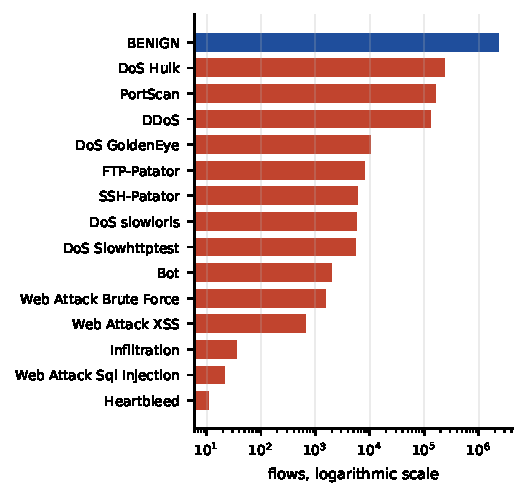
\includegraphics[width=\linewidth]{figures/class-balance.pdf}
  \caption{Flows per class on a logarithmic axis. Benign in blue, attacks in
  red. On a linear axis every family below the top three is invisible.}
  \label{fig:balance}
\end{figure}

\begin{figure}[t]
  \centering
  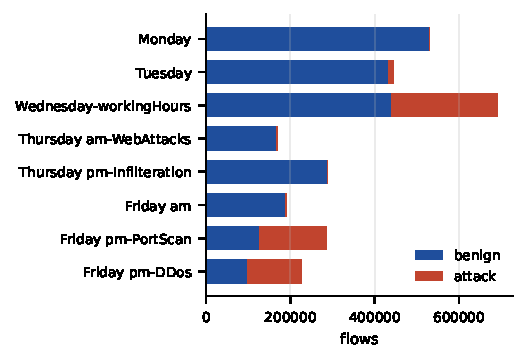
\includegraphics[width=\linewidth]{figures/session-mix.pdf}
  \caption{Benign and attack traffic per capture session. Monday is benign
  only and the attack share elsewhere swings from \SI{0.01}{\percent} to
  \SI{57}{\percent}.}
  \label{fig:sessions}
\end{figure}

\subsection{Cleaning and splitting}

Cleaning drops the padding rows, the infinities, \num{115} flows with a negative
duration and the eight dead columns, leaving \num{2827761} flows and 69
features. Only \texttt{Destination Port} is kept from the identity columns,
which matches the standard feature set; the rest travel alongside for display
and enrichment but are never given to a model.

A \num{60000} flow replay slice is taken out first, before the train and test
split, so nothing the dashboard streams was ever seen during fitting. The rest
is split 75 to 25, stratified on the attack family so the rare ones survive on
both sides. All three splits hold \SI{19.68}{\percent} attacks.

The replay slice is shuffled rather than ordered by capture time, and
Figure~\ref{fig:sessions} is why. Monday is benign only and accounts for a
fifth of the data, so a chronological replay spends its first quarter with
nothing to detect, while Wednesday and both Friday afternoon sessions are more
than a third attacks. Shuffling gives every second of the stream the attack
density of the capture as a whole. Chronological order remains available behind
a flag.

\subsection{Scaling}

Figure~\ref{fig:skew} explains the one preprocessing decision that is not
routine. The largest value of \texttt{Total Length of Bwd Packets} sits
\num{9125} times above its own 99th percentile, and nine other features are in
the same condition. Standardising such a column leaves a handful of flows
setting the scale for all of it, and the autoencoder loss becomes a report on
those few flows.

A quantile transform fixes this and was the first choice. It also cost
\SI{20}{\milli\second} to transform a single row, which was more than all three
models spent deciding put together. The final transform is
$\operatorname{sign}(x)\log(1+|x|)$ followed by standardisation: it compresses
the same tails, runs in microseconds, and is a plain array expression rather
than a library call with per invocation validation.

\begin{figure}[t]
  \centering
  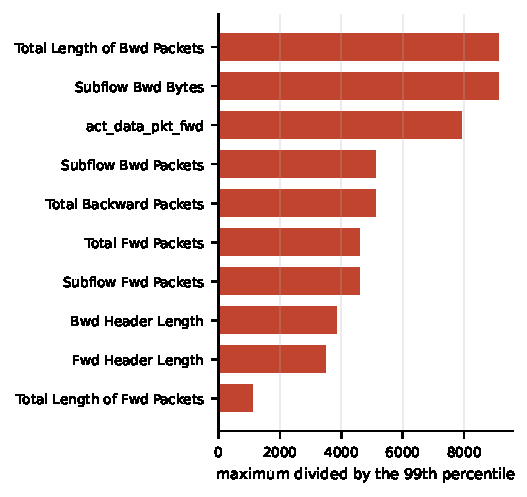
\includegraphics[width=\linewidth]{figures/feature-skew.pdf}
  \caption{Maximum value divided by the 99th percentile, for the ten heaviest
  tailed features.}
  \label{fig:skew}
\end{figure}

\section{Method}

\subsection{Fitting}

The random forest is fitted on the full training split with balanced subsample
class weights, and alerts above a probability of $0.5$.

The two unsupervised models never see an attack. Both are fitted on the
\num{1667258} benign flows of the training split, and both take their threshold
from the same rule: the quantile of their own score distribution on that benign
data corresponding to a \SI{1}{\percent} target false positive rate. Without a
shared rule they would be compared at whatever operating point their library
happened to default to.

\subsection{Serving}

All three sit behind one interface, so a number in the benchmark is produced by
the same code path that serves a live prediction. Two details matter for
latency. The tree ensembles drop to a single worker at serving time, because
handing one row to a thread pool costs more than scoring it; this alone took the
forest from \SI{17}{\milli\second} to \SI{3}{\milli\second} per flow. And the
scaler, described above, accounts for the rest.

\section{Hyperparameter study}

\subsection{How many trees}

Figure~\ref{fig:forest} shows recall between \SI{99.76}{\percent} and
\SI{99.78}{\percent} from five trees to two hundred, while the time to score one
flow rises from \SI{0.33}{\milli\second} to \SI{6.70}{\milli\second}. Every tree
past the first handful buys nothing and costs latency. The deployed forest was
reduced from 100 trees to 50, which halved the served latency from
\SI{3.09}{\milli\second} to \SI{1.66}{\milli\second} with no measurable change
in recall.

\begin{figure}[t]
  \centering
  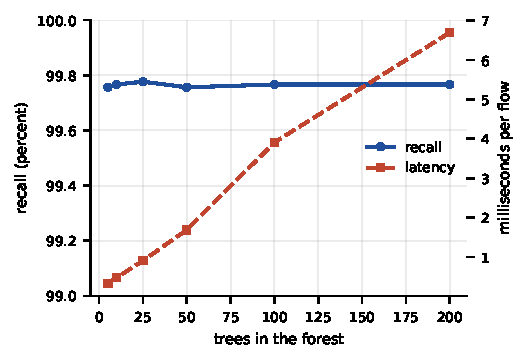
\includegraphics[width=\linewidth]{figures/forest-size.pdf}
  \caption{Random forest recall and per flow latency against the number of
  trees. The two lines do not agree.}
  \label{fig:forest}
\end{figure}

\subsection{How much each isolation tree sees}

Figure~\ref{fig:isolation} shows recall climbing monotonically with the number
of flows each tree is fitted on, from \SI{0.95}{\percent} at 128 samples to
\SI{17.0}{\percent} at \num{16384}. The scikit-learn default of 256 sits near
the worst end of that curve. Moving to \num{16384} took recall on the full test
split from \SI{11.3}{\percent} to \SI{17.2}{\percent} at the same false positive
rate.

\begin{figure}[t]
  \centering
  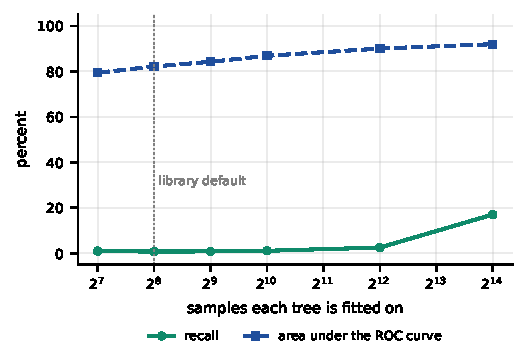
\includegraphics[width=\linewidth]{figures/isolation-samples.pdf}
  \caption{Isolation forest quality against samples per tree. The dotted line
  marks the library default.}
  \label{fig:isolation}
\end{figure}

\subsection{When to stop training the autoencoder}

Figure~\ref{fig:learning} is the argument for measuring detection quality every
epoch rather than only the loss. Over 25 epochs the reconstruction loss falls
steadily from $0.540$ to $0.036$, but the area under the ROC curve peaks at
epoch 7 at $0.932$ and then drifts back to $0.918$, while recall keeps climbing
until roughly epoch 16 and flattens. Training longer makes the reconstruction
better without making the detector better.

\begin{figure}[t]
  \centering
  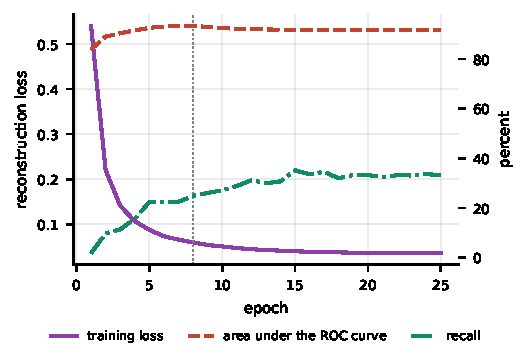
\includegraphics[width=\linewidth]{figures/learning-curve.pdf}
  \caption{Autoencoder loss, area under the ROC curve and recall by epoch. The
  dotted line marks the epoch of best ranking quality.}
  \label{fig:learning}
\end{figure}

\section{Results}

Table~\ref{tab:results} reports the three models on \num{691941} held out
flows, \num{136187} of them attacks.

\begin{table}[t]
  \centering
  \small
  \caption{Held out test split. Both unsupervised models are thresholded at a
  \SI{1}{\percent} target false positive rate.}
  \label{tab:results}
  \begin{tabular}{lrrrr}
    \toprule
    Model & Recall & FP rate & AUC & Latency \\
    \midrule
    Random Forest    & \SI{99.87}{\percent} & \SI{0.07}{\percent} & 1.000 & \SI{1.66}{\milli\second} \\
    Isolation Forest & \SI{17.24}{\percent} & \SI{1.01}{\percent} & 0.921 & \SI{3.29}{\milli\second} \\
    Autoencoder      & \SI{37.69}{\percent} & \SI{1.01}{\percent} & 0.930 & \SI{0.33}{\milli\second} \\
    \bottomrule
  \end{tabular}
\end{table}

Figure~\ref{fig:family} is the more informative view. The supervised model is
near perfect on every family with more than a thousand examples and drops to
\SI{81}{\percent} on Bot and \SI{67}{\percent} on Infiltration, the two rarest.
Those are the only two places where an unsupervised model competes: the
autoencoder reaches \SI{89}{\percent} on Infiltration. Neither unsupervised
model detects a port scan at all, because a port scan is a small, ordinary
looking flow, and asking whether a flow is unusual in general is not the same
question as asking whether it is unusual for its destination port.

\begin{figure}[t]
  \centering
  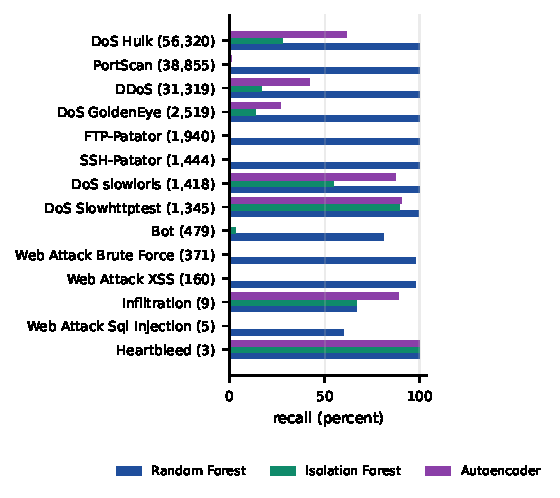
\includegraphics[width=\linewidth]{figures/per-family-recall.pdf}
  \caption{Recall per attack family, with the number of test flows in
  parentheses. Families are ordered by size.}
  \label{fig:family}
\end{figure}

Figure~\ref{fig:roc} shows the whole trade off rather than one point on it, and
Figure~\ref{fig:separation} shows why the autoencoder cannot do better at any
threshold: the benign and attack score distributions overlap heavily, and the
threshold is placed where it is only because the false positive budget says so.

\begin{figure}[t]
  \centering
  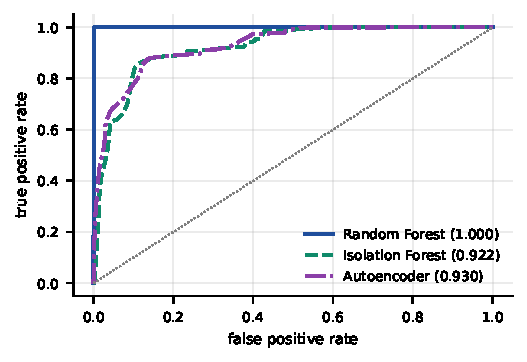
\includegraphics[width=\linewidth]{figures/roc-curves.pdf}
  \caption{ROC curves with the area under each in parentheses.}
  \label{fig:roc}
\end{figure}

\begin{figure}[t]
  \centering
  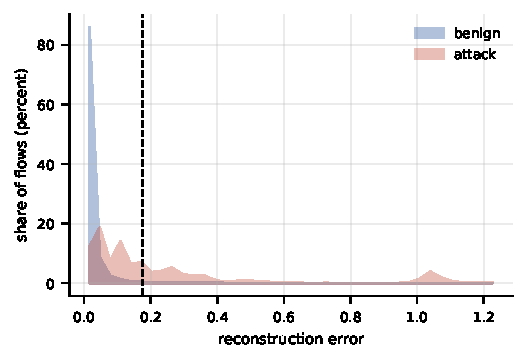
\includegraphics[width=\linewidth]{figures/score-separation.pdf}
  \caption{Autoencoder reconstruction error for benign and attack flows, each
  normalised to its own class. The dashed line is the threshold in use.}
  \label{fig:separation}
\end{figure}

\section{How much to trust the numbers}

\subsection{Leakage under a random split}

A denial of service burst produces thousands of flows identical in every
feature, so a random split puts copies of the same row on both sides. The
dataset holds \num{2497153} distinct feature vectors for \num{2827761} flows;
\SI{14.1}{\percent} of a random test split has a byte identical twin in the
training half, and \SI{27.8}{\percent} of the test attacks do.

Refitting under a split that trains on the earlier part of every capture session
and tests on the later part gives Table~\ref{tab:split}. The supervised model
barely moves and its false positive rate improves, so the duplicates are real
but they are not what produces the headline number. The unsupervised models lose
half their recall or more, and that is the useful finding: their thresholds are
fitted on the benign traffic of the training window, and benign traffic drifts
within a working day. Anything deployed this way needs its threshold
recalibrated on a rolling window rather than fixed once at training time.

\begin{table}[t]
  \centering
  \small
  \caption{Recall under a random split and under a time ordered split.}
  \label{tab:split}
  \begin{tabular}{lrr}
    \toprule
    Model & Random & Time ordered \\
    \midrule
    Random Forest    & \SI{99.9}{\percent} & \SI{98.5}{\percent} \\
    Isolation Forest & \SI{6.9}{\percent}  & \SI{1.8}{\percent} \\
    Autoencoder      & \SI{43.2}{\percent} & \SI{22.8}{\percent} \\
    \bottomrule
  \end{tabular}
\end{table}

\subsection{Attacks nobody trained on}

The supervised model works under a closed world assumption. To measure what
that costs, one family at a time was removed from training, all three models
refitted, and each asked about the family none of them was shown.

Figure~\ref{fig:novelty} did not come out the way an argument for an ensemble
usually goes, and the result is more useful than that argument would have been.
The supervised model does not degrade on an unseen family, it collapses on
three of six and holds up on the other three, and the pattern is whether a
structurally similar family remains in training. DDoS survives at
\SI{63.9}{\percent} because DoS Hulk is still there; slowloris survives at
\SI{89.8}{\percent} because the other slow denial of service families are; web
brute force survives at \SI{80.4}{\percent} because cross site scripting and SQL
injection are. PortScan, Bot and FTP-Patator have no close relative left and the
model goes to zero on all three.

The unsupervised models are not a safety net either. They recover
\SI{33.7}{\percent} on DDoS and \SI{32.2}{\percent} on slowloris, and nothing at
all on the other four.

\begin{figure}[t]
  \centering
  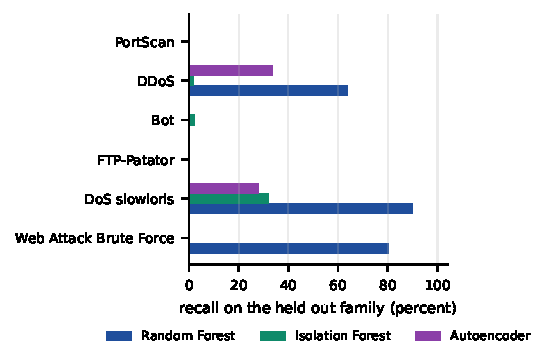
\includegraphics[width=\linewidth]{figures/novelty.pdf}
  \caption{Recall on a family removed from training. The unsupervised models
  see no attacks during training, so only the supervised one changes.}
  \label{fig:novelty}
\end{figure}

\section{Conclusion}

The supervised model is the one to deploy. It is accurate, it survives a
harder split, and at \SI{1.66}{\milli\second} per flow it keeps up with a
respectable link on one core. The two unsupervised models earn a narrower place:
they help on the rarest families, where labels are too few for supervision to
work, and they recover part of the loss on two of six unseen families.

What none of them does is handle a genuinely new attack. A system built on these
needs a retraining pipeline and human review, not a detector assumed to catch
the unknown. Three further directions follow from the measurements above rather
than from a wish list: recalibrating the unsupervised thresholds on a rolling
window, weighting the autoencoder reconstruction error per feature so that an
anomaly confined to one dimension is not averaged away across 69, and
conditioning the models on destination port so that ``unusual'' can mean
``unusual for this service''.

\section*{Reproducing this report}

Every figure and every number above comes from a command in the repository.

\begin{small}
\begin{verbatim}
python -m ids.data.download
python -m ids.data.explore --out reports
python -m ids.data.preprocess
python -m ids.train
python -m ids.benchmark
python -m ids.sweep
python -m ids.curves
python -m ids.validate
python -m ids.novelty
python -m ids.report.figures
\end{verbatim}
\end{small}

\noindent\small
Dataset: I. Sharafaldin, A. H. Lashkari and A. A. Ghorbani, \emph{Toward
Generating a New Intrusion Detection Dataset and Intrusion Traffic
Characterization}, ICISSP 2018.

\end{document}
